\section{Calendar}

Eftersom calendar skal have mulighed for at have personlig, samt fælles visning for en hel gruppe som widget, blev der besluttet at den personlige skulle være nem at navigere til, og er derfor blevet placeret i hjemmesidens navbar. Af denne grund er det blevet besluttet at lave to controllere, en GroupCalendar samt en Calendar til personlig visning. For at opsummere hvad kalenderens funktionalitet skal indebære, kan der herunder ses de user stories som calendar er en del af:

\begin{itemize}
    \item Tilføj/fjern begivenheder
    \item Valg af filter
    \item Skift mode (fælles/personlig)
    \item Valg af visning
    \item Mulighed for synkronisering med Google Calendar *
\end{itemize}

*Ikke implementeret

På nedenstående tabel ses, hvilken funktionalitet der er for begge kalendere.

%GroupCalendar laves som widget, og har derfor CRUD funktioner som den personlige ikke har, og den personlige har heller ikke mulighed for at indsætte events, da events skal tilknyttes en gruppe. \newline


\noindent  
\begin{tabular}{|p{2.0in}|p{1.5in}|p{1.5in}|} \hline 
\textbf{} & \textbf{Gruppe kalender} & \textbf{Personlig kalender}\\ \hline 
Overblik af en gruppes events & x & x \\ \hline
Overblik over events for alle grupper, bruger er medlem af &  & x \\ \hline 
Widget & x &  \\ \hline 
Tilf{\o}je begivenheder & x &  \\ \hline 
Slette begivenheder & x & \\ \hline 
Valg af visning & x & x \\ \hline
CRUD funktioner for widget & x &  \\ \hline
\end{tabular}
\noindent 



\subsection{Data view}

I første iteration af arbejdet med kalenderen blev der kun gemt events i databasen, eftersom det er det eneste som behøves i databasen for at få kalenderen til at virke. Alle events har gruppeID, og de kan på denne måde findes til hver gruppe på denne måde. Hvis systemet bliver populært, kan dette dog hurtigt blive et problem, at skulle iterere igennem alle events i hele databasen. I senere iterationer skulle kalenderen laves til widget, og der blev i denne forbindelse gemt en liste af events for hver calendar widget, hvori man så blot finder events ud fra denne liste. I bilag \cite{ArkitekturCalendar} kan der læses mere om dette, hvori der også kan ses data access layer.

\begin{figure}[H]
    \centering
    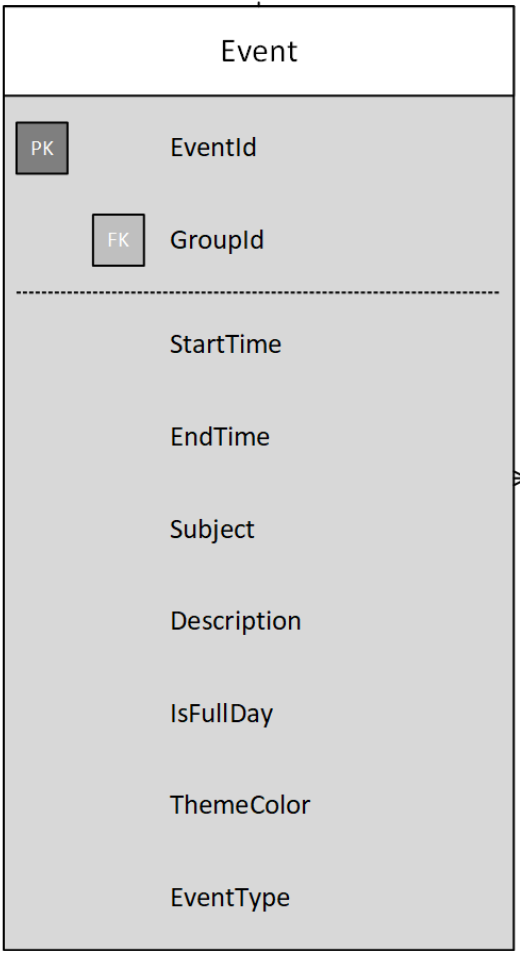
\includegraphics[width=0.25\linewidth]{09_Arkitektur/Calendar/Images/EventData.png}
    \caption{Event database model. Det kan ses GroupId er en foreign key, hvilket kan bruges til at finde de events der findes for en bestemt gruppe}
    \label{fig:eventDB}
\end{figure}

\subsection{Logical view}

Da der blev undersøgt hvordan der kunne laves en kalender, blev der fundet siden "fullcalendar.io", som er en populær javascript baseret kalender med fine stylesheets, og som gratis kan benyttes \cite{Fullcalendar}. fullcalendar.io har desuden valg af dag/uge/måned visning indbygget, hvilket er en user story for kalenderen. Hertil er der lavet et javascript "GroupCalendar.js", som henter events ned i kalenderen fra URL'en /GroupCalendar/GetEvents/(int id, string type), som er en action der returnerer et JSON result. Ud fra disse events, noteret på JSON format, så dannes kalenderen. 
For at overholde kravene noteret i user stories, er der derudover kommet frem til klassediagrammet i figur \ref{fig:CalendarControllerClass}.

\begin{figure}[H]
    \centering
    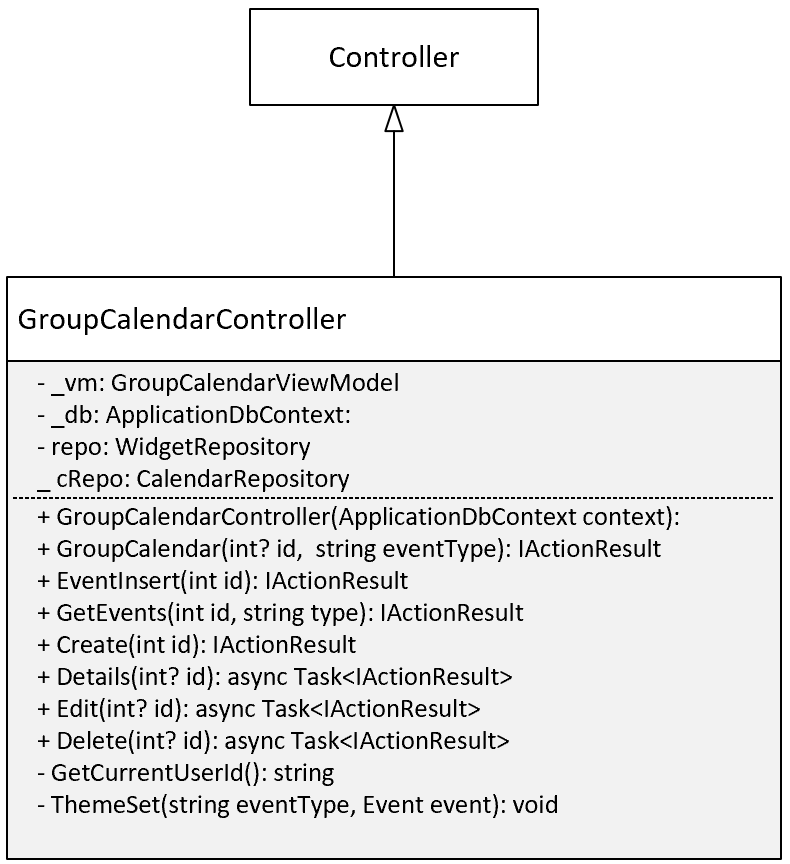
\includegraphics[width=0.5\linewidth]{09_Arkitektur/Calendar/Images/CalendarController.png}
    \caption{Figuren viser CalendarController klassediagrammet. Det ses at der er en GroupCalendarViewModel, som indeholder information til at danne URL'en som "GroupCalendar.js" henter events fra. Til Data Access Layer benyttes Widget og CalendarRepository }
    \label{fig:CalendarControllerClass}
\end{figure}{}

Hovedsageligt benyttes repository til DAL, bla. for at overholde SRP, men til små mindre kald til databasen, som ikke giver mening at lave en metode til i repository, benyttes ApplicationDbContext. \newline